%stpa

\documentclass[../../main/main.tex]{subfiles}


\begin{document}
\title{System-Theoretic Process Analysis}


\chapter{System-Theoretic Process Analysis}
\section{Systems Engineering}
\section{Systems Security Engineering}
\section{System-Theoretic Process Analysis}
The primary source for this section is the \glsentryshort{stpa} Handbook \cite{stpa}. It is referred to as the "handbook" in the remainder of this chapter.
\section{STPA Overview: Four Steps}
The four steps to the STPA process are briefly described below and then applied to the patrol base operations model in the next section.
\paragraph*{Step 1: Define The Purpose of The Analysis}
\paragraph*{Step 2: Model The Control Structure}
\paragraph*{Step 3: Identify Unsafe Control Actions}
\paragraph*{Step 4: Identify Loss Scenarios}

\section{STPA on Patrol Base Operations}
\subsection{Step 1: Define The Purpose of The Analysis}
\paragraph*{Define The Purpose of The Analysis}
The purpose of this analysis is to demonstrate the systems security engineering objective (as described by NIST Special Publication 800-160) of designing trustworthy systems with regards to complete mediation.  Complete mediation is the demonstrated outcome of applying the \glsentryshort{csbd} methodology to automated systems.  In this particular analysis, \glsentryshort{csbd} is applied to a non-automated, human-centered system exemplified by the U.S. Ranger Handbook's patrol base operations.  Thus, the more immediate goal is to demonstrate complete mediation in the patrol base operations.  A side-effect is a more thorough understanding of how access-control principals function in non-automated, human-centered military systems.  

\paragraph*{Identify Losses  with Regards to The Stakeholders}
Losses are defined with regards to stakeholders.  The stakeholders and identifiable losses are described below.

\begin{itemize}
\item U.S. Government\\
As a stakeholder, the U.S. Government is very much concerned with national security. Therefore, mission failure is a loss.
\item U.S. Army\\
The more immediate stake for the U.S. Army is successfully carrying out the mission.  Again, mission failure is a loss.
\item U.S. Intelligence Community\\
The U.S. intelligence community has a mission to gather intelligence that is critical for national security and mission success.  For reconnaissance missions, mission failure is a loss. For covert missions, discovery of the mission is a loss.  Also, capture of any personnel with sensitive information is a loss. 
\item U.S. military personnel and their families\\
The safety and well-being of military personnel is a concern for all stakeholders.  Nevertheless, it is the most immediate concern of the military personnel themselves.  Therefore, capture, morbidity, and morality are a loss.
\item U.S. Taxpayers\\
The most immediate concern for U.S. taxpayers is the cost war.  Therefore, equipment loss and damage are losses.  
\item U.S. Politicians\\
The immediate concern for all politicians is national security.  Therefore, mission failure is a loss.   In addition, politicians are often held accountable by the public for any actions taken by the U.S. military.  This means that negative publicity is a loss.  
\item Military Industrial Complex\\
The military industrial complex is a vital asset to national security and plays a critical role in the lives and safety of military personnel as well as United State's military superiority.  They have a stake in demonstrating the superiority of their equipment.  Therefore, equipment failure is a loss.  They also have a stake in demonstrating that their equipment provides U.S. war fighters with an edge in the battlefield.  Therefore, mission failure is a loss.
\item The enemy\\
The enemy has a stake in mission failure.  Their loss is considered a gain.  Therefore, mission failure is a loss.  
\item Regional peoples\\
Regardless of whether the patrol base operations are conducted in a foreign land or at home, preservation of culture, civilian lives, and resources are a concern.  Thus, disruption of the local culture and damage to resources is a loss. 
\end{itemize}


\subsection{Step 2: Model The Control Structure}
Defining the system boundaries: (reference Ranger Handbook)
One of the challenges in modeling the patrol base operations is generality.  Patrol base operations may consist of a fire team comprised of ? soldiers, a platoon comprised of ? soldiers, or something in-between.  The mission\footnote{Note that the Ranger Handbook specifically states that "because a patrol is an organization, not a mission, it is not correct to speak of giving a unit a mission to "patrol.""  The term "mission" used in this master thesis refers generally to the mission (or objectives) of the patrol base operations, and does not refer to the patrol as being a mission.}
 may be to engage with the enemy, to acquire intelligence for the main body, or some else.


Figure \ref{system} shows a diagram relating a system to its boundaries, subsystems, and inputs and outputs.  These each described below.

\begin{figure}[h]
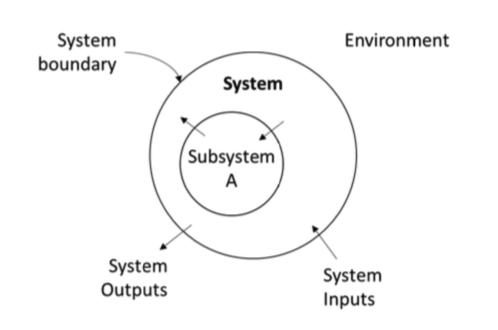
\includegraphics[width=\linewidth]{../figures/system}
\caption{\label{system}Relationship of system to system boundaries, subsystems, inputs, and outputs. (Image captured from the \glsentryshort{stpa} Handbook \cite{stpa}.)}
\end{figure}
\paragraph*{System}
In this master thesis, the "system" refers to a platoon-sized patrol base operation.  This is the best choice because a platoon-sized operation may be scaled-down to accommodate a squad-sized or fire team-sized detachment, but not the other way around. 

The mission details are intentionally kept vague to accommodate as many types of missions as possible.  The system boundaries for the model are the start and end of the mission. In this master thesis, the patrol base operations begin in the planning phase when the patrol leader receives the mission.  The patrol base operations end after the patrol withdraws from the operations and returns to the main body\footnote{Completion should include reporting to the commander.  However, for the purposes of this master thesis, it was sufficient to conclude a withdraw.  Nevertheless, with our model of the patrol base operations, it is easy to add a phase for reporting to the commander.}

\paragraph*{Subsystem}
A subsystem in the patrol base operations is any smaller group of soldier assigned to a specific task such as security or reconnaissance.  This may include a squad or fire team.  

\paragraph*{Environment}
The mission is determined by the greater-wisdom of the U.S. Army leadership at the time of need.  This means that environmental boundaries, mission boundaries, and other system requirements must be determined by the patrol leader  (referred to as the platoon leader in other chapters) after the mission is received and during the planning phase.  For this reason, STPA analysis should be performed on a mission before it is referred to the patrol.  But also, patrol leaders should be trained in STPA to make a quick and accurate analysis of mission-specific system boundaries.  


\paragraph*{System Inputs and Outputs}
The system input is the mission handed down by the U.S. Army leadership.  Additional inputs such as equipment, weapons, and additional personnel are determined when the mission is received. 

System outputs are mission dependent.  They may be successful engagement with the enemy, the capture of an enemy combatant, acquisition of specific intelligence, or anything else defined by the mission objectives.




\subsection{Step 3: Identify Unsafe Control Actions}
\subsection{Step 4: Identify Loss Scenarios}
\end{document}